\documentclass[12pt]{article}
\title{EE351K Homework 6}
\author{Hershal Bhave (hb6279)}
\date{Due October 16, 2014}

\usepackage{multicol}
\usepackage[in]{fullpage}
\usepackage{xcolor}
\usepackage{rotating}
\usepackage{mathtools}
\usepackage{amssymb}
\usepackage{cleveref}
\usepackage{graphics}
\usepackage{caption}
\usepackage{wrapfig}
\usepackage{subcaption}
\usepackage[nosolutionfiles]{answers}
\usepackage[acronym]{glossaries}

\newenvironment{Ex}{\textbf{Problem}\vspace{.75em}\\}{}
\Newassociation{solution}{Soln}{Answers}
\pagebreak[3]
\newcommand{\Opentesthook}[2]{\Writetofile{#1}{\protect\section{#1: #2}}}
\renewcommand{\Solnlabel}[1]{\textbf{Solution}\quad}

\newcommand{\dd}[1]{\:\mathrm{d}{#1}}
\newcommand{\ddt}[1]{\frac{\dd{}}{\dd{#1}}}
\newcommand{\dddt}[1]{\frac{\dd{}^2}{\dd{#1}^2}}

\begin{document}
\maketitle
\begin{enumerate}
\item
  \begin{Ex}
    Random Variables $X$ and $Y$ are described by the joint PDF
    \begin{equation}
      \label{eq:1-question}
      f_{X,Y}(x,y) = \left\{
        \begin{aligned}
          & ax &&\quad 2\le x\le 4,\quad 0\le y \le x \\
          & 0 &&\quad \text{otherwise} \\
        \end{aligned}\right.
    \end{equation}
    \begin{enumerate}
    \item Evaluate the constant $a$.
    \item Determine the marginal PDF $f_Y(y)$.
    \item Determine the expected value for $\frac{1}{X}$ given that $Y=3$.
    \end{enumerate}
    \begin{solution} \hfill
      \begin{enumerate}
      \item The constant $a$ can be determined by integrating across
        the area which $f_{X,Y}$ is defined and setting it equal to 1.
        \begin{equation}
          \label{eq:1a-presol}
          \begin{aligned}
            1 &= \int_0^x \int_2^4 ax \dd{x} \dd{y} \\
          \end{aligned}
        \end{equation}
        We can reverse the integrals to get an exact result
        \begin{equation}
          \label{eq:1a-sol}
          \begin{aligned}
            1 &= \int_2^4 \int_0^x ax \dd{y} \dd{x} \\
            &= a \int_2^4 x \int_0^x 1 \dd{y} \dd{x} \\
            &= a \int_2^4 x \; [y]_0^x \dd{x} \\
            &= a \int_2^4 x^2 \dd{x} \\
            &= a \left[\frac{x^3}{3}\right]_2^4 \dd{x} \\
            &= a \left(\frac{64}{3} - \frac{8}{3}\right) \\
            \implies a&=\frac{3}{56} \\
          \end{aligned}
        \end{equation}
      \item Marginals can be computed by the following
        \begin{equation}
          \label{eq:1b-marginal-def}
          f_Y(y) = \int_{-\infty}^{\infty} f_{X,Y}(x,y) \dd{x}
        \end{equation}
        So we can insert our PDF into this equation to obtain the
        proper marginal.
        \begin{equation}
          \label{eq:1b-sol}
          \begin{aligned}
            f_Y(y) &= \int_{y}^{4} ax \dd{x} \\
            &= a \int_{y}^{4} x \dd{x} \\
            &= a \left[\frac{x^2}{2}\right]_y^4 \\
            \implies f_Y(y) &= a \left(8 - \frac{y^2}{2}\right) \\
          \end{aligned}
        \end{equation}
        Which means that the marginal from 2 to 4 is $f_Y(y) =
        \frac{9}{28}$.
      \item The Expected Value in this situation can be calculated
        by
        \begin{equation}
          \label{eq:1c-expected-value}
          E[g(X)|Y=y] = \int_{-\infty}^{\infty} g(x)f_{X|Y}(x|y) \dd{x}
        \end{equation}
        where
        \begin{equation}
          \label{eq:1c-conditional-value}
          f_{X|Y}(x|y) = \frac{f_{X,y}(x,y)}{f_Y(y)}
        \end{equation}
        So the equation we need turns out to be
        \begin{equation}
          \label{eq:1c-sol}
          \begin{aligned}
            E\left[\frac{1}{X}|Y=3\right] &= \int_{3}^{4}
            \frac{1}{x} \frac{f_{X,Y}(x,y)}{f_Y(y)} \dd{x} \\
            &= \int_{3}^{4} \frac{1}{x} \frac{ax}{a\left(8 -
                \frac{y^2}{2}\right)} \dd{x} \\
            &= \int_{3}^{4} \frac{1}{x} \frac{x}{8 - \frac{3^2}{2}}
            \dd{x} \\
            &= \int_{3}^{4} \frac{1}{x} \frac{x}{\frac{7}{2}} \dd{x} \\
            &= \int_{3}^{4} \frac{1}{x} \frac{2x}{7} \dd{x} \\
            &= \int_{3}^{4} \frac{2}{7} \dd{x} \\
            \implies E\left[\frac{1}{X}|Y=3\right] &= \frac{2}{7} \\
          \end{aligned}
        \end{equation}
      \end{enumerate}
    \end{solution}
  \end{Ex}
\item
  \begin{Ex}
    Suppose $X$ and $Y$ are described by the joint PDF
    \begin{equation}
      \label{eq:2-question}
      f_{X,Y}(x,y) = \left\{
        \begin{aligned}
          &5x^2/2 &&\quad -1 \le x \le 1, \quad 0\le y \le x^2 \\
          &0 &&\quad \text{otherwise} \\
        \end{aligned} \right.
    \end{equation}
    Let $A$ be the event that $\{Y\le 1/3\}$
    \begin{enumerate}
    \item What is the conditional joint density $f_{X,Y|A}(x,y)$?
    \item What are $f_{Y|A}(y)$ and $f_{X|A}(x)$?
    \item What are $E[Y|A]$ and $E[X|A]$?
    \end{enumerate}
    \begin{solution} \hfill

      {\color{red}{\huge QUESTION}\\ If $Y$ is limited by $Y\le1/3$,
        and $Y$ is dependent on $X$, then does $X$ become limited as
        well?}

      \begin{enumerate}
      \item The way to obtain the conditional joint density is through
        the formula
        \begin{equation}
          \label{eq:2a-conditional-joint-density}
          f_{X,Y|A} = \left\{
            \begin{aligned}
              & \frac{f_{X,Y}(x,y)}{P(A)} &&\quad(x,y) \in A \\
              & 0 &&\quad\text{otherwise} \\
            \end{aligned} \right.
        \end{equation}
        In order to use that though, we must obtain the CDF for
        $P(A)$, where
        \begin{equation}
          \label{eq:2a-cdf}
          P(A) = P(Y \le y) = \int_{-\infty}^{y} f_{Y}(y) \dd{y}
        \end{equation}
        Which we must obtain the marginal $f_Y(y)$ in order to use. We
        will do that now
        \begin{equation}
          \label{eq:2a-marginal}
          \begin{aligned}
            F_Y(y) &= \int_{-\infty}^{\infty} f_{X,Y}(x,y) \dd{x} \\
            &= \int_{-1}^1 \frac{5x^2}{2} \dd{x} \\
            &= \frac{5}{2} \int_{-1}^{1} x^2 \dd{x} \\
            &= \frac{5}{2} \left[\frac{x^3}{3}\right]_{-1}^1 \\
            &= \frac{5}{2} \frac{2}{3} \\
            \implies F_Y(y) &= \frac{5}{3} \\
          \end{aligned}
        \end{equation}
        Now we can plug that into \cref{eq:2a-cdf}:
        \begin{equation}
          \label{eq:2a-cdf-plugged}
          \begin{aligned}
            P(Y \le y) &= \int_{-\infty}^{y} f_{Y}(y) \dd{y} \\
            P\left(Y \le \frac{1}{3}\right) &=
            \int_{0}^{\frac{1}{3}} \frac{5}{3} \dd{y} \\
            &= \frac{5}{3} \int_{0}^{\frac{1}{3}} 1 \dd{y} \\
            &= \frac{5}{3} \; [y]_0^{\frac{1}{3}} \\
            &= \frac{5}{3} \frac{1}{3} \\
            \implies P\left(Y \le \frac{1}{3}\right) &= \frac{5}{9} \\
          \end{aligned}
        \end{equation}
        So now we can obtain the conditional joint density
        \begin{equation}
          \label{eq:2a-conditional-joint-density-plugged}
          \begin{aligned}
            f_{X,Y|A}(x,y) &= \frac{f_{X,Y}(x,y)}{P(Y \le 1/3)} \\
            &= \frac{\frac{5x^2}{2}}{\frac{5}{9}} \\
            \implies f_{X,Y|A}(x,y) &= \frac{9x^2}{2} \\
          \end{aligned}
        \end{equation}
        Or, more precisely
        \begin{equation}
          \label{eq:2a-sol}
          \implies f_{X,Y|A}(x,y) = \left\{
            \begin{aligned}
              & \frac{9x^2}{2} &&\quad (x,y) \in A \\
              & 0 && \text{otherwise} \\
            \end{aligned}\right.
        \end{equation}
      \item{\color{red}{\huge TODO}}
      \item{\color{red}{\huge TODO}}
      \end{enumerate}
    \end{solution}
  \end{Ex}
\item
  \begin{Ex}
    Suppose $X$ has PDF:
    \begin{equation}
      \label{eq:3-question}
      f_X(x) = \left\{
        \begin{aligned}
          &\frac{x}{2} &&\quad 0\le x\le 2 \\
          &0 &&\quad \text{otherwise} \\
        \end{aligned}\right.
    \end{equation}
    Where $X$ denotes the length of a stick. Now suppose the stick is
    randomly broken and let $Y$ denote the length of the remaining
    stick.
    \begin{enumerate}
    \item Find the joint PDF of $Y$ and $X$.
    \item Find the marginal PDF of $Y$.
    \item Find $E[Y]$.
    \end{enumerate}
    \begin{solution} \hfill
      \begin{enumerate}
      \item $Y$ is conditional on $X$ where $X$ represents the length
        of the stick with the PDF described in \cref{eq:3-question},
        and $Y$ represents the length of the remaining stick after it
        is randomly broken. We can represent the process of ``randomly
        breaking'' the stick by a uniform distribution dependent on
        $X$:
        \begin{equation}
          \label{eq:3a-y-given-x-dist}
          \begin{aligned}
            f_{Y|X}(y|x) \sim \text{Uniform}[0,x], \text{ given } X = x
          \end{aligned}
        \end{equation}
        Which can then be written as
        \begin{equation}
          \label{eq:3a-y-given-x-pdf}
          \implies f_{Y|X}(y|x) = \left\{
            \begin{aligned}
              & \frac{1}{x} &&\quad 0 \le y \le x \\
              & 0 &&\quad \text{otherwise} \\
            \end{aligned} \right.
        \end{equation}
        We can then write the PDF as the following
        \begin{equation}
          \label{eq:3a-presol}
            f_{X,Y}(x,y) = f_X(x)f_{Y|X}(y|x)
        \end{equation}
        Which we can then precisely write as
        \begin{equation}
          \label{eq:3a-sol}
          \implies f_{X,Y}(x,y) = \left\{
            \begin{aligned}
              & \frac{1}{2} &&\quad 0 \le x \le 2,
              \quad 0 \le y \le x \\
              & 0 &&\quad\text{otherwise} \\
            \end{aligned} \right.
        \end{equation}
      \item The general equation for computing the marginal PDF of $Y$
        is given as
        \begin{equation}
          \label{eq:3b-general-marginal}
          f_Y(y) = \int_{-\infty}^{\infty} f_{X,Y}(x,y) \dd{x}
        \end{equation}
        We will use this to calculate the desired marginal for $Y$.
        \begin{equation}
          \label{eq:3b-sol}
          \begin{aligned}
            f_Y(y) &= \int_{-\infty}^{\infty} f_{X,Y}(x,y) \dd{x} \\
            &= \int_{y}^{2} \frac{1}{2} \dd{x} \\
            &= \left[\frac{x}{2}\right]_y^2 \\
            \implies f_Y(y) &= 1 - \frac{y}{2} \\
          \end{aligned}
        \end{equation}
      \item Calculating the expected value is done by integrating the
        marginal $f_Y(y)$ multiplied by $y$.
        \begin{equation}
          \label{eq:3c-sol}
          \begin{aligned}
            E[Y] &= \int_{-\infty}^{\infty} y f_Y(y) \dd{y} \\
            &= \int_{0}^{2} y(1-\frac{y}{2}) \dd{y} \\
            &= \int_{0}^{2} y-\frac{y^2}{2} \dd{y} \\
            &= \left[\frac{y^2}{2}-\frac{y^3}{6}\right]_{0}^{2}
            \dd{y} \\
            &= 2-\frac{4}{3} \\
            \implies E[Y] &= \frac{2}{3} \\
          \end{aligned}
        \end{equation}
      \end{enumerate}
    \end{solution}
  \end{Ex}
\item
  \begin{Ex}
    A customer entering a store is served by clerk $i$ with
    probability $p_i$, where $i = 1,\ldots,n$. The time taken by clerk
    $i$ to serve a customer is an exponentially distributed random
    variable with parameter $\alpha_i$.
    \begin{enumerate}
    \item Find the PDF of $T$, the time taken to service a customer.
    \item Find $E[T]$ and $\text{Var}(T)$. You should find expressions
      in terms of $p_i$ and $\alpha_i$, where $i = 1,\ldots,n$
    \item Suppose $T > 5$. Find an expression for the probability that
      clerk $i$ served the customer. Hint: You will need to use a
      version of Bayes Rule.
    \end{enumerate}
    \begin{solution} \hfill \\\\ {\huge TODO}
    \end{solution}
  \end{Ex}
\item
  \begin{Ex}
    Suppose $X = e^Y$ where $Y\sim \text{Normal}(\mu, \sigma^2)$, i.e.
    \begin{equation}
      \label{eq:5-question}
      f_Y(y) =
      \frac{1}{\sqrt{2\pi\sigma^2}}e^{-\frac{(y-\mu)^2}{2\sigma^2}}
      \quad\text{for }-\infty < y < \infty
    \end{equation}
    then $X$ is said to have a log normal distrubtion with parameters
    $\mu$, $\sigma^2$, denoted $X \sim
    \text{Lognormal}(\mu,\sigma^2)$. Determine the PDF of $X$.
    \begin{solution} \hfill \\\\ {\huge TODO}
    \end{solution}
  \end{Ex}
\item
  \begin{Ex}
    A mixed RV is a ``mixture'' of a discrete and a continuous RV. FOr
    example, suppose $X$ is discrete with CDF $F_X(x)$ and $Y$ is
    continuous with CDF $F_Y(y)$. Define:
    \begin{equation}
      \label{eq:6-question}
      Z = \left\{
        \begin{aligned}
          & X &&\quad \alpha \\
          & Y &&\quad (1-\alpha) \\
        \end{aligned} \right.
      \quad\quad\alpha \in [0,1].
    \end{equation}
    $Z$ is said to be a mixed RV.
    \begin{enumerate}
    \item Suppose $X \sim \text{Bernoulli}(p)$, $Y\sim
      \text{exp}(\lambda)$, and $\alpha=\frac{1}{2}$. Find the CDF of
      $Z$.

    \item Suppose $Z$ has CDF $F_Z(z)$ described in
      \cref{fig:6-fig}. Find $F_X$ discrete, $F_Y$ continuous, and
      $\alpha$ for $Z$.
      % \begin{wrapfigure}{r}{0.5\textwidth}
      %   \begin{center}
      %     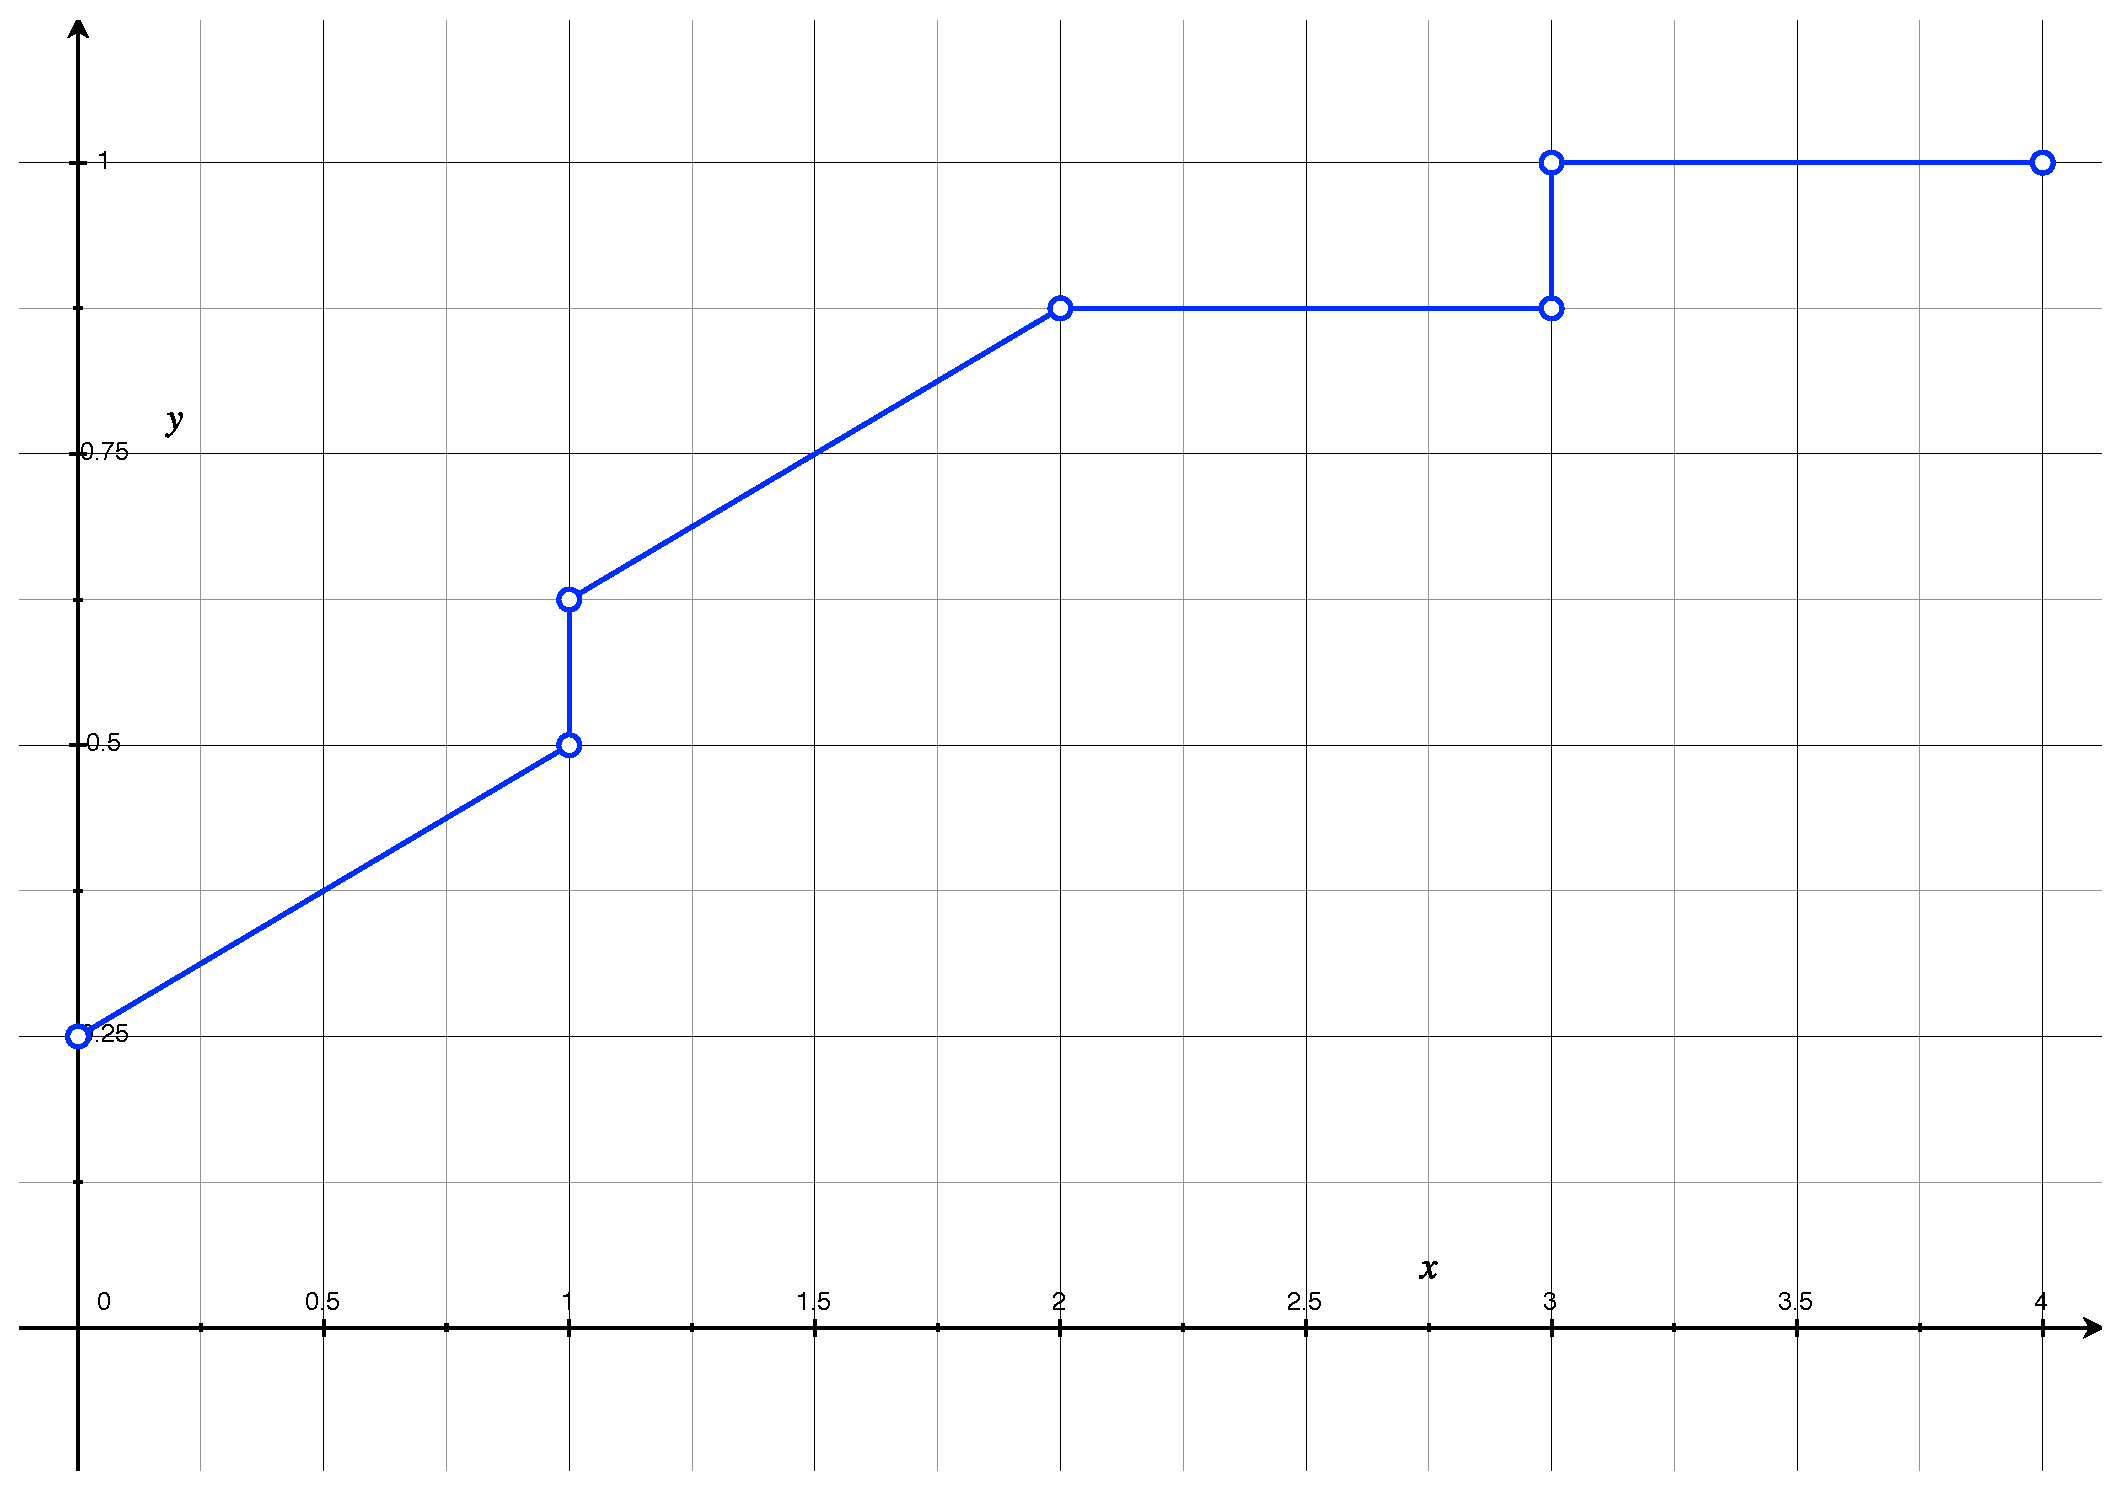
\includegraphics[width=0.48\textwidth]{6-fig}
      %   \end{center}
      %   \caption{$F_Z(z)$}
      %   \label{fig:6-fig}
      % \end{wrapfigure}
      \begin{figure}[h]
        \centering
        \resizebox{.95\textwidth}{!}{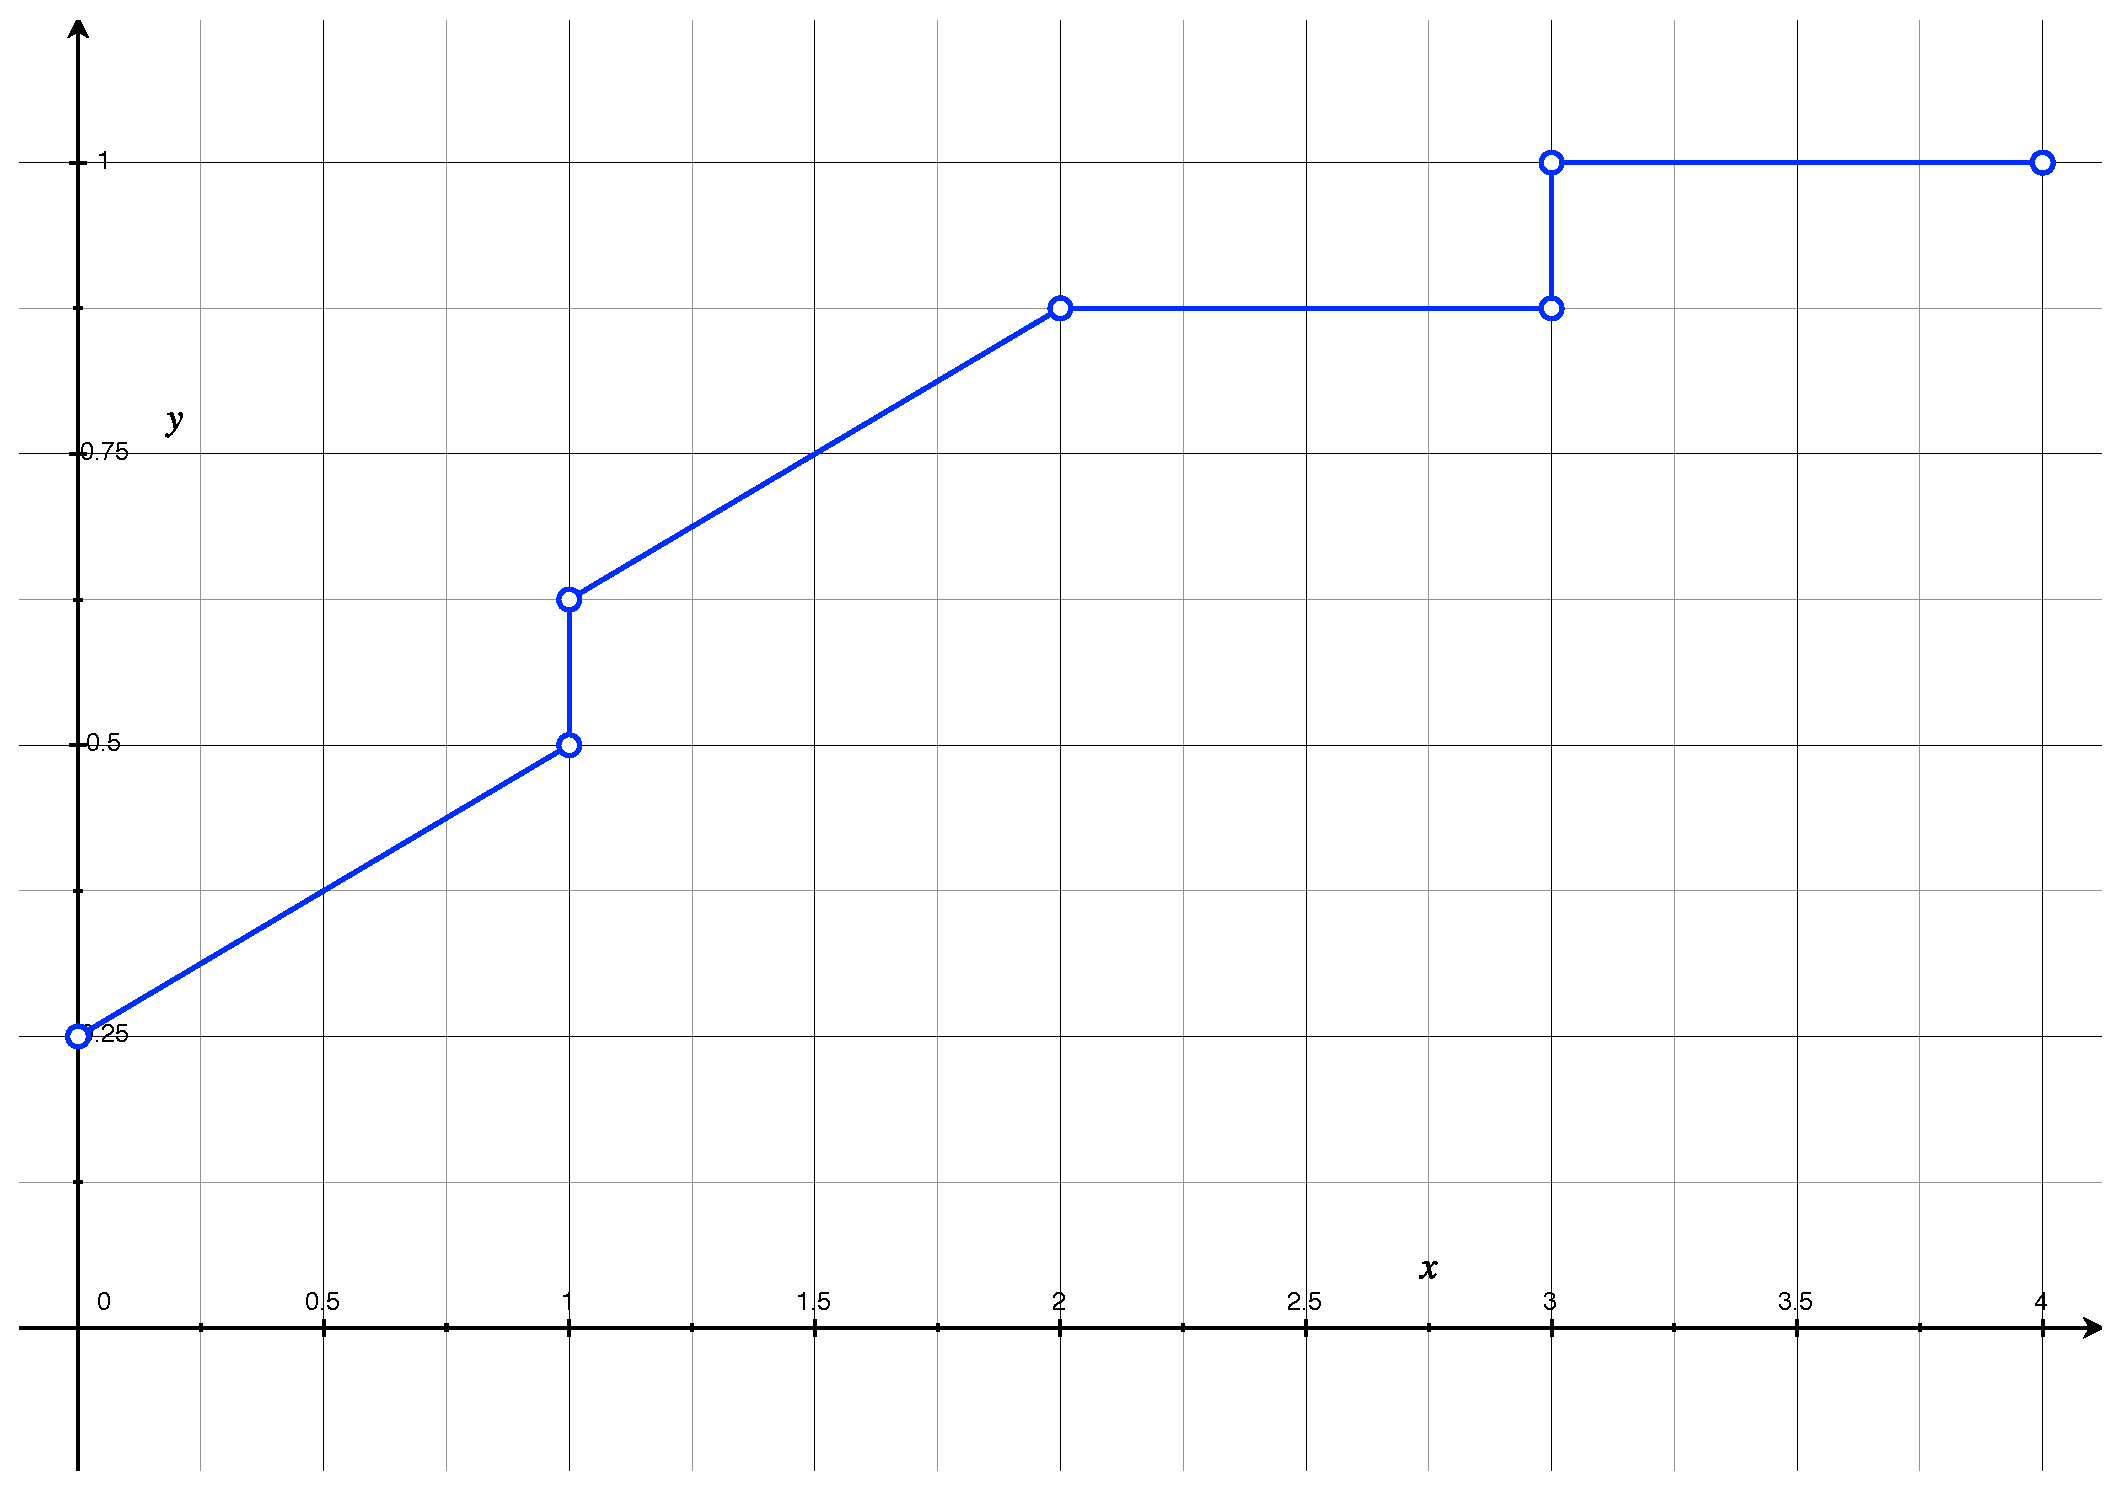
\includegraphics{6-fig}}
        \caption{$F_Z(z)$}
        \label{fig:6-fig}
      \end{figure}
    \end{enumerate}
    \begin{solution} \hfill \\\\ {\huge TODO}
    \end{solution}
  \end{Ex}
\item
  \begin{Ex}
    Jane goes to the bank to make a withdrawal, and is equally likely
    to find 0 or 1 customers ahead of her. The service time of the
    customer ahead, if present, is exponentially distributed with
    parameter $\lambda$ What is the CDF of Jane’s waiting time?
    \begin{solution} \hfill \\\\ {\huge TODO}
    \end{solution}
  \end{Ex}

\end{enumerate}
\end{document}
